\documentclass[conference]{IEEEtran}
\IEEEoverridecommandlockouts
\usepackage{amsmath,amssymb,amsfonts}
\usepackage{amsthm}
\usepackage{graphicx}
\usepackage{booktabs}
\usepackage{xcolor}
\usepackage{cite}
\usepackage{tikz}
\usetikzlibrary{positioning,arrows.meta,fit}
\usepackage[hidelinks]{hyperref}

\newtheorem{proposition}{Proposition}
% Red notes would mark results still being computed; none remain.
\newcommand{\todo}[1]{\textcolor{red}{[TODO: #1]}}

% All numbers below come from paper/generated/tables.tex, produced by `python -m bixrec.make_tables`.
% generated by bixrec.make_tables -- do not edit by hand
\newcommand{\resMlOneSasrecNdcg}{--}
\newcommand{\resMlOneSasrecHr}{--}
\newcommand{\resMlOnePoeNdcg}{--}
\newcommand{\resMlOnePoeHr}{--}
\newcommand{\resMlOnePoeFiftyNdcg}{--}
\newcommand{\resMlOnePoeFiftyHr}{--}
\newcommand{\resMlOneHybridNdcg}{--}
\newcommand{\resMlOneHybridHr}{--}
\newcommand{\resMlOneLateNdcg}{--}
\newcommand{\resMlOneLateHr}{--}
\newcommand{\resMlOneBixNdcg}{--}
\newcommand{\resMlOneBixHr}{--}
\newcommand{\resMlOneTextNdcg}{--}
\newcommand{\resMlOneTextHr}{--}
\newcommand{\gainMlOnePoe}{--}
\newcommand{\gainMlOneHybrid}{--}
\newcommand{\gainMlOneSasrec}{--}
\newcommand{\gainMlOneLate}{--}
\newcommand{\resBeautySasrecNdcg}{--}
\newcommand{\resBeautySasrecHr}{--}
\newcommand{\resBeautyPoeNdcg}{--}
\newcommand{\resBeautyPoeHr}{--}
\newcommand{\resBeautyPoeFiftyNdcg}{--}
\newcommand{\resBeautyPoeFiftyHr}{--}
\newcommand{\resBeautyHybridNdcg}{--}
\newcommand{\resBeautyHybridHr}{--}
\newcommand{\resBeautyLateNdcg}{--}
\newcommand{\resBeautyLateHr}{--}
\newcommand{\resBeautyBixNdcg}{--}
\newcommand{\resBeautyBixHr}{--}
\newcommand{\resBeautyTextNdcg}{--}
\newcommand{\resBeautyTextHr}{--}
\newcommand{\gainBeautyPoe}{--}
\newcommand{\gainBeautyHybrid}{--}
\newcommand{\gainBeautySasrec}{--}
\newcommand{\gainBeautyLate}{--}
\newcommand{\resSportsSasrecNdcg}{--}
\newcommand{\resSportsSasrecHr}{--}
\newcommand{\resSportsPoeNdcg}{--}
\newcommand{\resSportsPoeHr}{--}
\newcommand{\resSportsPoeFiftyNdcg}{--}
\newcommand{\resSportsPoeFiftyHr}{--}
\newcommand{\resSportsHybridNdcg}{--}
\newcommand{\resSportsHybridHr}{--}
\newcommand{\resSportsLateNdcg}{--}
\newcommand{\resSportsLateHr}{--}
\newcommand{\resSportsBixNdcg}{--}
\newcommand{\resSportsBixHr}{--}
\newcommand{\resSportsTextNdcg}{--}
\newcommand{\resSportsTextHr}{--}
\newcommand{\gainSportsPoe}{--}
\newcommand{\gainSportsHybrid}{--}
\newcommand{\gainSportsSasrec}{--}
\newcommand{\gainSportsLate}{--}
\newcommand{\tabMain}{
\begin{table*}[t]
\centering
\caption{Full-catalog leave-one-out results (no negative sampling), mean\,$\pm$\,sd over seeds, in \%. Best per column in bold.}
\label{tab:main}
\small
\begin{tabular}{lcccccc}
\toprule
 & \multicolumn{2}{c}{ML-1M} & \multicolumn{2}{c}{Beauty} & \multicolumn{2}{c}{Sports} \\
\cmidrule(lr){2-3} \cmidrule(lr){4-5} \cmidrule(lr){6-7}
Model & HR@10 & NDCG@10 & HR@10 & NDCG@10 & HR@10 & NDCG@10 \\
\midrule
SASRec (ID) & -- & -- & -- & -- & -- & -- \\
Text expert & -- & -- & -- & -- & -- & -- \\
Static PoE ($\alpha{=}0.5$) & -- & -- & -- & -- & -- & -- \\
Tuned PoE ($\alpha$ on val.) & -- & -- & -- & -- & -- & -- \\
Early fusion (ID + text) & -- & -- & -- & -- & -- & -- \\
Joint late fusion & -- & -- & -- & -- & -- & -- \\
\midrule
BiXRec (full) & -- & -- & -- & -- & -- & -- \\
\bottomrule
\end{tabular}
\end{table*}
}
\newcommand{\tabSig}{
\begin{table}[t]
\centering
\caption{BiXRec against each baseline: mean relative change of NDCG@10 over seeds, seeds won, two-sided Wilcoxon signed-rank test on per-user NDCG@10 averaged over seeds (Holm-adjusted over all rows), and the largest per-seed exact McNemar $p$ on HR@10.}
\label{tab:sig}
\small
\begin{tabular}{llrcrr}
\toprule
Data & Baseline & $\Delta$NDCG & Wins & $p_\mathrm{Holm}$ & $\max p_\mathrm{McN}$ \\
\midrule
\multicolumn{6}{c}{-- results pending --} \\
\bottomrule
\end{tabular}
\end{table}
}
\newcommand{\tabAbl}{
\begin{table}[t]
\centering
\caption{Ablation (NDCG@10, \%, mean\,$\pm$\,sd). Static PoE fuses two separately trained experts; all other rows are trained end to end with the same loss and budget.}
\label{tab:ablation}
\small
\begin{tabular}{lccc}
\toprule
Variant & ML-1M & Beauty & Sports \\
\midrule
Static PoE ($\alpha{=}0.5$) & -- & -- & -- \\
Joint late fusion & -- & -- & -- \\
Joint late fusion + penalty & -- & -- & -- \\
+ cross-attention & -- & -- & -- \\
+ cross-attention + gate & -- & -- & -- \\
BiXRec (full) & -- & -- & -- \\
\bottomrule
\end{tabular}
\end{table}
}
\newcommand{\tabAudit}{
\begin{table}[t]
\centering
\caption{Training-protocol audit (NDCG@10, \%). ``Last position only'' and ``BCE + 1 negative'' reproduce the training choices of our earlier pipeline.}
\label{tab:audit}
\small
\begin{tabular}{lccc}
\toprule
Variant & ML-1M & Beauty & Sports \\
\midrule
SASRec, last position only & -- & -- & -- \\
SASRec, BCE + 1 negative & -- & -- & -- \\
SASRec (ID) & -- & -- & -- \\
BiXRec, last position only & -- & -- & -- \\
BiXRec (full) & -- & -- & -- \\
\bottomrule
\end{tabular}
\end{table}
}
\newcommand{\tabMask}{
\begin{table*}[t]
\centering
\caption{Effect of removing history items from the ranking (NDCG@10, \%). Because repeated user--item pairs are removed, the target is never in the history and masking can only help.}
\label{tab:mask}
\small
\begin{tabular}{lcccccc}
\toprule
 & \multicolumn{2}{c}{ML-1M} & \multicolumn{2}{c}{Beauty} & \multicolumn{2}{c}{Sports} \\
Model & unmasked & masked & unmasked & masked & unmasked & masked \\
\midrule
SASRec (ID) & -- & -- & -- & -- & -- & -- \\
Tuned PoE ($\alpha$ on val.) & -- & -- & -- & -- & -- & -- \\
Early fusion (ID + text) & -- & -- & -- & -- & -- & -- \\
BiXRec (full) & -- & -- & -- & -- & -- & -- \\
\bottomrule
\end{tabular}
\end{table*}
}
\newcommand{\tabLength}{
\begin{table*}[t]
\centering
\caption{NDCG@10 (\%) by history-length tercile of the test users (short / medium / long), averaged over seeds.}
\label{tab:length}
\small
\begin{tabular}{llcccc}
\toprule
Data & Tercile (len.) & SASRec & Tuned PoE & Early fusion & BiXRec \\
\midrule
\bottomrule
\end{tabular}
\end{table*}
}
\newcommand{\tabOverlap}{
\begin{table}[t]
\centering
\caption{Hit overlap at HR@10 of the separately trained ID expert (C) and text expert (S), mean over seeds. $n_{11}$: both hit; $n_{10}$: only C; $n_{01}$: only S. A per-user selector between C and S gains at most $n_{01}$ hits over C and puts $n_{10}$ at risk; base rate $=n_{01}/(n_{01}+n_{10})$.}
\label{tab:overlap}
\small
\begin{tabular}{lrrrrrr}
\toprule
Data & Users & $n_{11}$ & $n_{10}$ & $n_{01}$ & Base rate & BiXRec $-$ C \\
\midrule
\bottomrule
\end{tabular}
\end{table}
}
\newcommand{\tabData}{
\begin{table}[t]
\centering
\caption{Dataset statistics after 5-core filtering and removal of repeated user--item pairs.}
\label{tab:data}
\small
\begin{tabular}{lrrrrr}
\toprule
Data & Users & Items & Inter. & Avg.\ len. & Density \\
\midrule
\multicolumn{6}{c}{-- generated after data preparation --} \\
\bottomrule
\end{tabular}
\end{table}
}


\begin{document}

\title{Where Should Collaborative and Semantic Experts Meet?\\
Score Routing versus Bilateral Cross-Attention in Sequential Recommendation}

\author{\IEEEauthorblockN{Anonymous Submission}}

\maketitle

\begin{abstract}
Sequential recommenders increasingly combine a collaborative expert over item IDs with a semantic expert over item
content. The usual recipe keeps the two experts separate and merges their scores, either with a static rule or with
a learned per-user router. We first give a model-free argument that bounds what any per-user selection between two
experts can gain: at most the users that only the semantic expert hits, and only if the selector is right on more
than half of the users it moves. On two Amazon datasets the measured base rate is 14\%, so routing has little to
gain. We
then ask whether the experts should instead meet inside their representations. BiXRec is a dual-stream transformer
in which an ID stream and a content stream exchange information at every layer through gated bilateral
cross-attention and are scored jointly with a candidate-level disagreement penalty. Every model in our study shares
one implementation, loss (full-softmax cross-entropy at all positions), budget and stopping rule, and a jointly
trained late-fusion control separates the effect of cross-attention from that of joint training. On MovieLens-100K,
where item content is a title, a year and genres, BiXRec improves NDCG@10 over SASRec by \gainMlHundredSasrec\% and
over early fusion by \gainMlHundredHybrid\% (Holm-corrected $p<0.05$), while its \gainMlHundredPoe\% over a tuned
product of experts is not significant with 943 test users. On Amazon Beauty and Sports, where content is a
handful of category and brand attributes, BiXRec beats the joint late-fusion control on every seed
(\gainBeautyLate\% and \gainSportsLate\%), and an ablation attributes this to cross-attention, but simple early
fusion is better on both (BiXRec \gainBeautyHybrid\% and \gainSportsHybrid\%), and on Sports BiXRec does not
improve on SASRec. Cross-attention therefore
pays off when item content is informative and is not a substitute for early fusion when it is not. A
training-protocol audit shows that training on the last position only cuts SASRec's NDCG@10 by about 75\%, a
larger effect than any fusion design we compare.
\end{abstract}

\begin{IEEEkeywords}
sequential recommendation, multimodal fusion, cross-attention, product of experts, routing, full-catalog evaluation
\end{IEEEkeywords}

% ---------------------------------------------------------------------------
\section{Introduction}

Collaborative sequential recommenders such as GRU4Rec, SASRec and BERT4Rec~\cite{hidasi2016gru4rec,kang2018sasrec,%
sun2019bert4rec} learn item transitions from interaction IDs and are strong when histories and item counts are
dense. Content encoders, from TF-IDF to Sentence-BERT~\cite{reimers2019sbert}, describe items from their text or
attributes, independently of interactions, and help where IDs are sparse. A common way to combine the two is late fusion: train a collaborative expert~$C$ and a
semantic expert~$S$ separately, then merge their scores, either statically (a weighted sum or a product of
experts~\cite{hinton2002poe}) or with a learned router that picks, per user, the expert that should be
trusted~\cite{shazeer2017moe,ma2018mmoe}.

The router idea is intuitive, and it is supported by a large oracle gap: choosing the better expert per user
afterwards beats any static rule by a wide margin. We argue that this gap is mostly unreachable. If both experts are
reasonable, most users that $S$ ranks correctly are also ranked correctly by $C$; the users that only $S$ gets right
are few, and they are mixed with a larger group that only $C$ gets right. Section~\ref{sec:bound} turns this into a
simple bound on what any per-user selector can gain and a break-even precision it must reach.

If choosing between finished scores cannot help much, the experts must exchange information earlier. We study a
direct design, BiXRec: two transformer streams, one over ID embeddings and one over projected content embeddings, that
query each other at every layer through gated bilateral cross-attention, in the spirit of co-attention in
vision--language models~\cite{lu2019vilbert}, and are scored jointly with a penalty on candidates on which the two
streams disagree.

Comparisons between fusion designs are easily confounded. Training on the last position only or with one sampled
negative, rather than full-softmax cross-entropy over all positions, changes the accuracy of sequential models by
large factors~\cite{klenitskiy2023dross,petrov2023gsasrec}; sampled evaluation changes model
rankings~\cite{krichene2020sampled,dallmann2021sampling}. A new fusion architecture trained with a stronger
objective than its baselines can look better for reasons unrelated to fusion. We therefore hold everything except
the fusion design fixed, and we add a control that is trained end to end exactly like BiXRec but without
cross-attention.

\textbf{Contributions.}
(i)~A model-free selection bound for two-expert late fusion, computed from the hit overlap of the experts, which
explains why per-user routing over frozen ID and text experts has little headroom (Sec.~\ref{sec:bound}).
(ii)~BiXRec, a dual-stream sequential recommender with gated bilateral cross-attention and a candidate-level
disagreement penalty (Sec.~\ref{sec:model}).
(iii)~A controlled evaluation with one implementation and one training protocol for all models, a joint-training
control, full-catalog ranking, history-masking and history-length analyses, and Holm-corrected paired tests
(Sec.~\ref{sec:setup}--\ref{sec:results}). It shows that the benefit of cross-attention depends on how informative
item content is: it wins with titles and genres, and loses to early fusion with sparse attribute tags.
(iv)~A training-protocol audit that quantifies the accuracy lost to two common shortcuts, as a reproducibility
lesson for fusion studies (Sec.~\ref{sec:audit}). Code, configurations, per-run metrics and per-user ranks are
released.

% ---------------------------------------------------------------------------
\section{Related Work}

\textbf{Sequential recommendation.} GRU4Rec~\cite{hidasi2016gru4rec}, SASRec~\cite{kang2018sasrec} and
BERT4Rec~\cite{sun2019bert4rec} are standard ID-based backbones. Replicability studies show that their relative
order depends strongly on the training objective: SASRec trained with full-softmax cross-entropy matches or beats
BERT4Rec~\cite{petrov2022bert4rec,klenitskiy2023dross}, and negative sampling makes models
overconfident~\cite{petrov2023gsasrec}.

\textbf{Side information and text.} FDSA~\cite{zhang2019fdsa} runs separate self-attention over items and features
and concatenates the results; S3-Rec~\cite{zhou2020s3rec} uses attributes for self-supervised pre-training;
NOVA~\cite{liu2021nova} and DIF-SR~\cite{xie2022difsr} inject side information into the attention computation
without mixing it into item representations. UniSRec~\cite{hou2022unisrec} and Recformer~\cite{li2023recformer}
learn transferable representations from item text. BiXRec differs in keeping two complete streams that exchange
information in both directions at every layer and are scored jointly; it is closest to FDSA (two streams) and to
co-attention~\cite{lu2019vilbert} (bilateral exchange).

\textbf{Combining experts.} Products of experts add log-probabilities~\cite{hinton2002poe}; mixtures of experts
learn input-dependent weights~\cite{shazeer2017moe,ma2018mmoe}. Choosing a predictor per instance is algorithm
selection~\cite{rice1976algorithm} or learning to defer~\cite{mozannar2020defer}. Our bound applies to any per-user
selector between two fixed rankers.

\textbf{Evaluation.} We rank against the full catalog~\cite{krichene2020sampled,dallmann2021sampling} and keep
validation and test targets out of training; global temporal leakage in leave-one-out
splits~\cite{ji2023leakage} remains and is discussed in Sec.~\ref{sec:limits}.

% ---------------------------------------------------------------------------
\section{Setting and the Selection Bound}\label{sec:bound}

Let $\mathcal{U}$ be the users, $\mathcal{I}$ the items and $s_u = (v_1,\dots,v_{n_u})$ the chronological history of
user $u$. A model scores every item given a prefix; the test target $v_{n_u}$ is ranked against the whole catalog,
and $\mathrm{hit}_u(M)=\mathbb{1}[\mathrm{rank}_M(v_{n_u})\le K]$.
Given experts $C$ and $S$, let $n_{11}$, $n_{10}$ and $n_{01}$ be the numbers of test users hit by both, by $C$ only
and by $S$ only.

\begin{proposition}\label{prop:bound}
For any selector $\pi:\mathcal{U}\to\{C,S\}$ that returns, per user, the ranking of one expert, and any set
$\mathcal{M}=\{u:\pi(u)=S\}$ of moved users,
\[
\textstyle\sum_u \mathrm{hit}_u(\pi)-\sum_u\mathrm{hit}_u(C)
= |\mathcal{M}\cap\mathcal{U}_{01}| - |\mathcal{M}\cap\mathcal{U}_{10}| \;\le\; n_{01},
\]
where $\mathcal{U}_{01}$ ($\mathcal{U}_{10}$) are the users hit only by $S$ (only by $C$). The selector improves on
$C$ only if more than half of the moved users that matter (those in $\mathcal{U}_{01}\cup\mathcal{U}_{10}$) are in
$\mathcal{U}_{01}$, whereas a selector without information about the outcome reaches the base rate
$n_{01}/(n_{01}+n_{10})$.
\end{proposition}
\begin{proof}
Users hit by both or by neither contribute the same hit under $\pi$ and $C$. A moved user in $\mathcal{U}_{01}$ gains
one hit, a moved user in $\mathcal{U}_{10}$ loses one. The maximum is reached for $\mathcal{M}=\mathcal{U}_{01}$.
\end{proof}

The bound covers routing between finished rankings. It does not cover rules that build a new score per candidate,
such as a product of experts or BiXRec, which can hit users that neither expert hits. Table~\ref{tab:overlap}
reports the overlap of our separately trained experts. On Beauty only 234 users are hit by the content expert
alone, against 1,486 hit by SASRec alone, and on Sports 239 against 1,434: a selector that has no information about
the outcome is right on 14\% of the users it moves, far below the 50\% it needs to break even, and even a perfect
selector could add at most 1\% of users. On MovieLens-100K the two groups are of similar size (48 and 50 users), so the base rate is close to
break-even and the bound is less restrictive, but the ceiling is again small (5\% of users). This is why we do not
pursue per-user routing and turn to fusion inside the representations.

\tabOverlap

% ---------------------------------------------------------------------------
\section{BiXRec}\label{sec:model}

\begin{figure}[t]
\centering
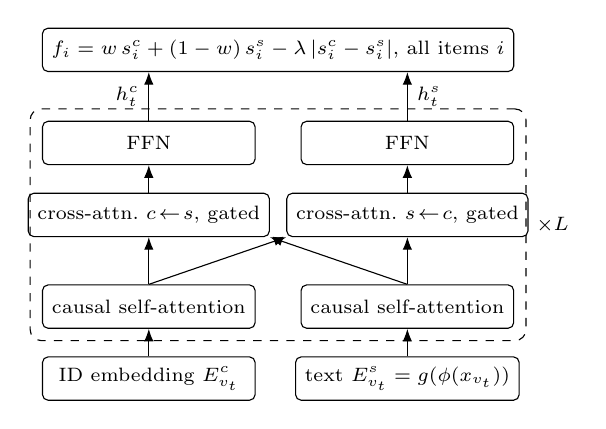
\begin{tikzpicture}[font=\scriptsize, node distance=3.5mm and 5mm,
  box/.style={draw, rounded corners=2pt, align=center, minimum width=27mm, minimum height=5.5mm},
  arr/.style={-{Latex[length=1.6mm]}}]
\node[box] (ec) {ID embedding $E^c_{v_t}$};
\node[box, right=of ec] (es) {text $E^s_{v_t}=g(\phi(x_{v_t}))$};
\node[box, above=of ec] (sc) {causal self-attention};
\node[box, above=of es] (ss) {causal self-attention};
\node[box, above=6mm of sc] (xc) {cross-attn.\ $c\!\leftarrow\!s$, gated};
\node[box, above=6mm of ss] (xs) {cross-attn.\ $s\!\leftarrow\!c$, gated};
\node[box, above=of xc] (fc) {FFN};
\node[box, above=of xs] (fs) {FFN};
\node[draw, dashed, rounded corners, fit=(sc)(ss)(fc)(fs), inner sep=1.5mm] (L) {};
\node[anchor=west, font=\scriptsize] at (L.east) {$\times L$};
\path (fc) -- (fs) coordinate[midway] (mid);
\node[box, minimum width=58mm, above=9mm of mid] (score) {$f_i = w\,s^c_i + (1-w)\,s^s_i - \lambda\,|s^c_i-s^s_i|$, all items $i$};
\draw[arr] (ec) -- (sc); \draw[arr] (es) -- (ss);
\draw[arr] (sc) -- (xc); \draw[arr] (ss) -- (xs);
\draw[arr] (ss.north) -- (xc.south east); \draw[arr] (sc.north) -- (xs.south west);
\draw[arr] (xc) -- (fc); \draw[arr] (xs) -- (fs);
\draw[arr] (fc.north) -- node[left]{$h^c_t$} (fc.north |- score.south);
\draw[arr] (fs.north) -- node[right]{$h^s_t$} (fs.north |- score.south);
\end{tikzpicture}
\caption{BiXRec. Two streams over the same item sequence exchange information at every layer and are scored jointly.}
\label{fig:arch}
\end{figure}

\textbf{Two streams.} For a prefix $(v_1,\dots,v_t)$ the collaborative stream embeds items with a learned table
$E^c\in\mathbb{R}^{|\mathcal{I}|\times d}$ and the semantic stream with $E^s_i = g(\phi(x_i))$, where $\phi$ is a
frozen content encoder applied to the item text or attributes $x_i$ and $g$ a two-layer MLP. Each stream adds its own positional
embeddings: $c^{(0)}_t=\sqrt{d}\,E^c_{v_t}+P^c_t$ and $s^{(0)}_t=\sqrt{d}\,E^s_{v_t}+P^s_t$.

\textbf{Gated bilateral cross-attention.} Each of the $L$ layers applies pre-norm causal self-attention to each
stream, then lets each stream attend to the other under the same causal and padding mask,
\begin{align*}
\tilde c &= \mathrm{XAttn}\big(\mathrm{LN}(c),\mathrm{LN}(s)\big),\\
\gamma^c &= \sigma\big(W^c[\mathrm{LN}(c);\tilde c]+b^c\big),\qquad c \leftarrow c + \gamma^c\odot\tilde c,
\end{align*}
and symmetrically for $s$, followed by a position-wise feed-forward network per stream. The gate bias is
initialised at zero, so each stream starts by injecting half of the cross-attention output; the gate can learn to
suppress text information where it is noisy, or ID information where IDs are rare.

\textbf{Joint scoring.} With final states $h^c_t,h^s_t$, every item $i$ receives
$s^c_i=\langle h^c_t,E^c_i\rangle$, $s^s_i=\langle h^s_t,E^s_i\rangle$ and
\begin{equation}
f_i = w\,s^c_i + (1-w)\,s^s_i - \lambda\,|s^c_i-s^s_i|,\label{eq:score}
\end{equation}
with $w=\sigma(\alpha)$ and $\lambda=\lambda_{\max}\sigma(\beta)$ learned ($\lambda_{\max}=0.35$; $\alpha=0$ and
$\beta=-1.5$ at initialisation). For $s^c_i>s^s_i$, Eq.~\eqref{eq:score} equals
$(w-\lambda)s^c_i+(1-w+\lambda)s^s_i$, and the other branch is symmetric: the stream that is more enthusiastic about a
candidate is down-weighted, which discounts items favoured by only one stream. With $\lambda=0$ the score is a
learned linear blend.

\textbf{Training.} All parameters except $\phi$ are trained end to end with full-softmax cross-entropy at every
position of every training sequence, $\mathcal{L}=-\sum_u\sum_{t}\log\mathrm{softmax}(f^{(u,t)})_{v_{t+1}}$, the
objective that gives SASRec its strongest results~\cite{klenitskiy2023dross}. The extra cost over two independent
SASRec-style encoders is two cross-attention modules and two gates per layer.

% ---------------------------------------------------------------------------
\section{Experimental Setup}\label{sec:setup}

\textbf{Datasets.} MovieLens-100K~\cite{harper2015movielens}, in the release distributed with
RecBole~\cite{zhao2021recbole}, whose item content is the title, release year and genres; and Amazon
Beauty and Sports \& Outdoors~\cite{mcauley2015image} in the 5-core releases of S3-Rec~\cite{zhou2020s3rec}, whose
item content is a set of anonymised category and brand attribute identifiers (on average 3--4 per item). The
datasets therefore span rich and poor item content. We apply an iterative 5-core filter, order interactions by time (ties by file order) and
keep the first occurrence of every user--item pair, so the test target never appears in the input history
(Table~\ref{tab:data}).

\tabData

\textbf{Protocol.} Leave-one-out per user: the last item is the test target, the second-to-last the validation
target, and all earlier items form the training sequence. No user group is treated differently. We rank the target
against all items without negative sampling and report HR@10 and NDCG@10; ties count against the target. The main
tables do not remove history items from the ranking; Table~\ref{tab:mask} reports both.

\textbf{Content encoder.} $\phi$ is TF-IDF over the item's text or attribute tokens followed by a truncated SVD to
128 dimensions (latent semantic analysis), fitted on item content only and frozen for every model. It uses no
interaction data and no pre-training corpus, so it cannot leak information about the test interactions; a
pre-trained sentence encoder is a drop-in replacement in our code.

\textbf{Models.} All models use the same transformer block (pre-norm, causal and key-padding masks), $d=64$, two
layers, two heads, maximum length 200 and dropout 0.2 on MovieLens-100K, and maximum length 50 and dropout 0.5 on
the Amazon datasets. \emph{SASRec}~\cite{kang2018sasrec}: ID stream only. \emph{Content expert}: content stream only, no IDs.
\emph{Static PoE}: separately trained SASRec and content expert fused as $\alpha\log p^C+(1-\alpha)\log p^S$, with
$\alpha=0.5$ or $\alpha\in\{0,0.05,\dots,1\}$ tuned on validation NDCG@10. \emph{Early fusion}: one stream whose item
embedding is $E^c_i+E^s_i$. \emph{Joint late fusion}: BiXRec without cross-attention, i.e.\ two streams that never
interact before Eq.~\eqref{eq:score} but are trained end to end through it. Ablations add the penalty,
cross-attention and the gate one at a time.

\textbf{Training.} AdamW~\cite{loshchilov2019adamw} (learning rate $10^{-3}$, $\beta_2=0.98$, no weight decay), batch
size 128, gradient clipping at 5, full-softmax cross-entropy at all positions for every model, at most 100 epochs,
and early stopping on validation NDCG@10 with patience 10, never before epoch 30; the test targets are used once,
after model selection. Seeds $\{42,123,2024\}$ change initialisation and batch order, and each seed retrains every
model. All runs were made on a 2-core CPU, which is what limits the number of epochs and seeds.

\textbf{Statistics.} Seeds share users, so we treat users as the unit of inference: for each model we average the
per-user NDCG@10 over seeds and compare BiXRec with each baseline by a two-sided Wilcoxon signed-rank test, with
Holm correction~\cite{holm1979} over all baseline--dataset pairs. We also report the number of seeds won and the
largest per-seed exact McNemar $p$ on HR@10~\cite{mcnemar1947}, a deliberately conservative check.

% ---------------------------------------------------------------------------
\section{Results}\label{sec:results}

\tabMain
\tabSig

\subsection{Overall accuracy}
Table~\ref{tab:main} reports accuracy and Table~\ref{tab:sig} the paired tests. On MovieLens-100K BiXRec has the
highest HR@10 and NDCG@10 (\resMlHundredBixNdcg\% NDCG@10, against \resMlHundredSasrecNdcg\% for SASRec,
\resMlHundredPoeNdcg\% for tuned PoE and \resMlHundredHybridNdcg\% for early fusion). Its gains over SASRec
(\gainMlHundredSasrec\%) and over early fusion (\gainMlHundredHybrid\%) are significant after Holm correction; its
gains over tuned PoE (\gainMlHundredPoe\%) and over joint late fusion (\gainMlHundredLate\%) are not, and the
seed-to-seed standard deviation (0.6 NDCG points) is of the same size as these gaps. With 943 test users,
MovieLens-100K can only detect large effects.

On the Amazon datasets the picture changes. Early fusion is the best model on both, and BiXRec is below it on
every seed (\gainBeautyHybrid\% on Beauty, \gainSportsHybrid\% on Sports, both significant). On Beauty BiXRec
improves on SASRec (\gainBeautySasrec\%), on static PoE with $\alpha=0.5$ and on joint late fusion
(\gainBeautyLate\%), all significant and on every seed, and matches tuned PoE. On Sports it beats joint late fusion
(\gainSportsLate\%, significant, every seed) but only matches SASRec (\gainSportsSasrec\%, not significant) and is
below tuned PoE (\gainSportsPoe\%, significant). The content expert alone is weak on both (HR@10 below 2\%), and
the dual-stream models learn to put most of the weight on the ID stream ($w\approx0.9$ for joint late fusion,
$w\approx0.8$ for BiXRec, against $w\approx0.54$ on MovieLens-100K). When item content is a few attribute
tags, adding it to the ID embedding is more useful than running a second stream over it, and a second stream can
even cost accuracy: joint late fusion is at or below SASRec on both Amazon datasets.

\subsection{Where does the gain come from?}
\tabAbl
The ablation in Table~\ref{tab:ablation} adds, in order, joint training (static PoE $\rightarrow$ joint late fusion),
the disagreement penalty, cross-attention and the gate. On MovieLens-100K no single component produces a clear step:
each partial model lies within one standard deviation of joint late fusion, and only the full combination is
higher than all of them; the learned penalty weight is small but consistent ($\lambda\approx0.07$--$0.08$ on every
seed). On Beauty the attribution is clear. We compare consecutive rows with the same per-user Wilcoxon test as
above, Holm-corrected over the ten step comparisons on both datasets. Adding cross-attention to joint late fusion is
the one step that matters on its own: $+0.11$ NDCG points ($p_\mathrm{Holm}=0.002$), on every seed. The penalty
alone ($+0.03$) and the gate alone ($-0.03$) change nothing measurable, and adding the penalty on top of gated
cross-attention gives a further $+0.06$ ($p_\mathrm{Holm}=0.04$). Overall, BiXRec is $0.14$ points above joint late
fusion on Beauty ($p_\mathrm{Holm}<0.001$). On MovieLens-100K no step survives the correction; the largest
is again the penalty on top of gated cross-attention ($+0.38$ points, $p_\mathrm{Holm}=0.08$). Cross-attention,
not joint training, is therefore what lifts BiXRec above late fusion when the effect is measurable, and the penalty
helps only in combination with it. We did not run the ablation on Sports.

\subsection{Relation to the selection bound}
The last column of Table~\ref{tab:overlap} gives the hits BiXRec adds over SASRec. On MovieLens-100K BiXRec adds 16
hits, a third of the 48 that an oracle selector could add; on Beauty it adds 40 hits, which no selector working at the
measured 14\% base rate could deliver, since such a selector loses hits. On Sports BiXRec has 15 hits fewer than
SASRec, although an oracle selector could add 239. Candidate-level fusion is not limited by the bound, because it can
rank targets that neither expert ranks in its top 10, but escaping the bound does not guarantee a gain.

\subsection{Who benefits?}
\tabLength
Table~\ref{tab:length} splits test users into terciles of history length. On MovieLens-100K BiXRec gains most on
the shortest histories (6.76\% NDCG@10 against 5.85\% for SASRec) and also leads on medium histories; on the longest
histories tuned PoE is slightly ahead. On both Amazon datasets early fusion is best in every tercile except the
medium Sports tercile, where tuned PoE leads; BiXRec is above SASRec in every Beauty tercile, and on Sports it is level
with SASRec on short and long histories and below it on medium ones. The gate is meant to help short histories, and this is where BiXRec's advantage on MovieLens-100K is
largest, but the ablation shows the gate alone does not explain it.

\subsection{History masking}
\tabMask
Removing history items from the ranking can only improve the rank of the target here, and it raises every model
substantially (NDCG@10 rises by 69--84\% on MovieLens-100K and by 32--37\% on the Amazon datasets). On the Amazon
datasets the order of the models is essentially unchanged (on Sports it is identical; on Beauty only SASRec and joint
late fusion, which differ by 0.02 points, swap). On MovieLens-100K, whose users have long histories, masking reorders the fusion models: joint
late fusion, tuned PoE and BiXRec end within 0.2 NDCG points of each other, so BiXRec's lead under the unmasked
protocol partly comes from ranking already-watched movies lower. Fusion studies should report both protocols.

\subsection{Training-protocol audit}\label{sec:audit}
\tabAudit
Table~\ref{tab:audit} trains SASRec and BiXRec on MovieLens-100K with two shortcuts. Training on the last position of
each sequence only reduces SASRec's NDCG@10 from 4.03\% to 1.02\% ($-75\%$) and BiXRec's from 4.81\% to 1.83\%
($-62\%$). Binary cross-entropy with one sampled negative reduces SASRec to 3.01\% ($-25\%$). These effects are an
order of magnitude larger than any difference between fusion designs in Table~\ref{tab:main}: a BiXRec trained with
the full objective would appear 372\% better than a SASRec trained on the last position only. Fusion models and their
baselines must be trained with the same objective.

% ---------------------------------------------------------------------------
\section{Discussion and Limitations}\label{sec:limits}

\textbf{What the evidence supports.} Per-user routing between frozen ID and content experts has a small ceiling and,
when the content expert is weak, a base rate far below break-even. Fusion inside the representations helps when
item content is informative (MovieLens-100K). With attribute tags (Beauty, Sports) BiXRec is consistently better
than an equally trained late-fusion control, but it is not better than early fusion, and on Sports not better than
SASRec. On Beauty, where the ablation has power, the gain over late fusion comes from cross-attention, and the
disagreement penalty helps only on top of it; on MovieLens-100K no single component is significant, and part of the
gain disappears when watched items are masked.

\textbf{Limitations.} (i)~Compute: all runs used a 2-core CPU, which limited us to three seeds, at most 100 epochs
and compact models with one shared hyper-parameter setting; tuning each model separately could change close
comparisons. (ii)~Content: we use a frozen TF-IDF/LSA encoder; Amazon content is anonymised attribute identifiers,
not product text, and MovieLens-100K is small. Pre-trained sentence encoders, product titles and larger datasets
such as MovieLens-1M are the natural next step, and the released code supports them unchanged. (iii)~The bound in
Sec.~\ref{sec:bound} applies to per-user selection between two finished rankings; it says nothing about learned
candidate-level rules. (iv)~Leave-one-out splits share a global timeline, so training sequences of some users may
contain interactions that happen after other users' test targets~\cite{ji2023leakage}. (v)~Seeds share the same
test users; per-user tests account for user variability but not for every source of training variance.
(vi)~Text-pre-trained recommenders such as UniSRec or Recformer~\cite{hou2022unisrec,li2023recformer} are not
compared.

\section{Conclusion}
Choosing, per user, between an ID expert and a content expert has little room to help, and the room shrinks as the
content expert weakens. Inside a dual-stream transformer, letting the streams exchange information through
cross-attention is consistently better than keeping them apart until the score, and this is what BiXRec adds. Whether
a second stream is worth having at all depends on the content: with titles and genres BiXRec is the best model we
tested, but with a few attribute tags simple early fusion wins on both datasets and BiXRec is at best a little better
than SASRec. The largest effect we measured is not a fusion design but the training objective, which must be held
fixed for fusion comparisons to mean anything.

\bibliographystyle{IEEEtran}
\bibliography{references}

\end{document}
